\section{3 October 2024 - Lab equipment}

The goal of the first lab experience was to get to know the lab equipment and how it works. Below are two pictures (Fig. \ref{fig:01_instruments} and \ref{fig:01_cables}) of the available equipment during this experience. Three resistors (\SI{100}{ohm}, \SI{470}{ohm}, and \SI{1000}{ohm}) were also available and were used at the end of the experience.
\begin{figure}[htbp]
	\centering
	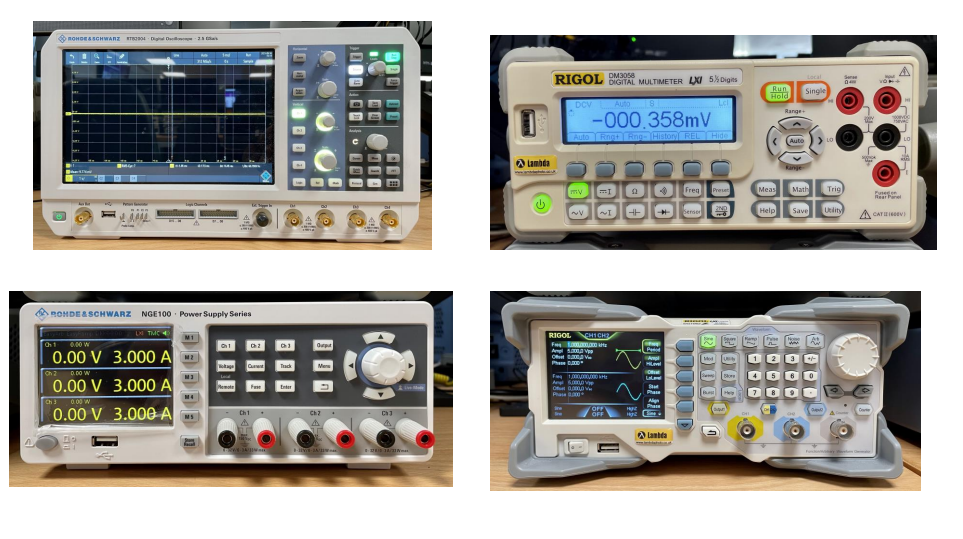
\includegraphics[width=0.6\textwidth]{lab_01/instruments.png}
	\caption{From top-left, in clockwise direction: the oscilloscope used to analyze signals, a DC power supply, an AC generator, and a digital multimeter used to measure resistances.}
	\label{fig:01_instruments}
\end{figure}
\begin{figure}[htbp]
	\centering
	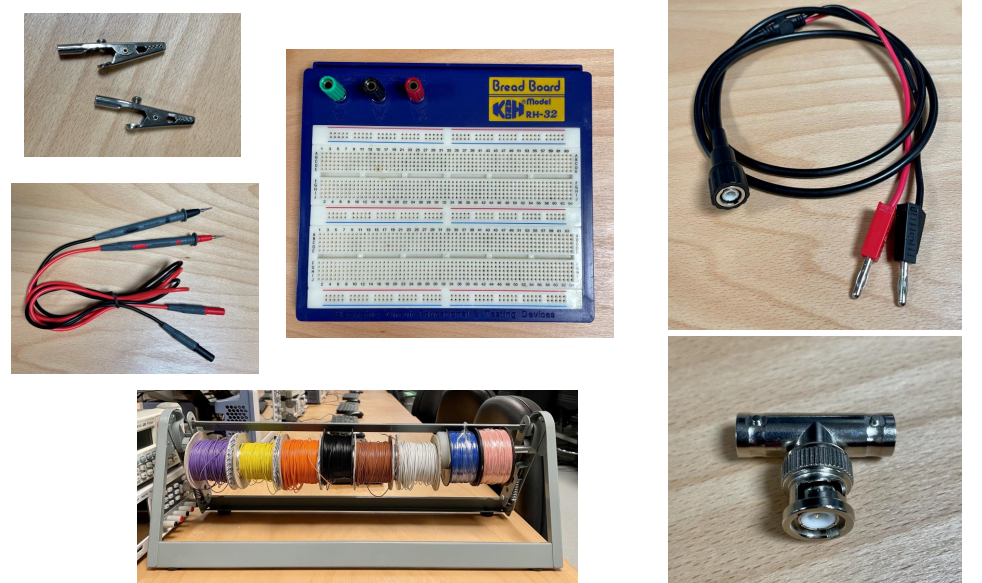
\includegraphics[width=0.6\textwidth]{lab_01/cables.png}
	\caption{From top-left, in clockwise direction: clips, a breadboard to build circuits on, banana cables, a connector, utility cables and DMM cables.}
	\label{fig:01_cables}
\end{figure}

\subsection{AC generator and the oscilloscope}